\documentclass[12pt,a4paper]{article} 
\pdfoutput=1
\usepackage{jheppub} 
\usepackage{graphicx} 
\usepackage{amsmath} 
\usepackage{amssymb} 
\usepackage{slashed} 
\usepackage{bigstrut} 
\usepackage{mathtools} 
\usepackage{multirow} 
%cmv added for the bibliography with strange characters:
\usepackage[utf8]{inputenc}
%\usepackage{lineno}
\usepackage{todonotes}
\usepackage{xspace}
\usepackage{lscape}
%\usepackage{rotating}
%\usepackage{afterpage}
%cmv

\newcommand{\msbar}{\ensuremath{\overline{\rm MS}}\xspace}
\newcommand{\dz}{\ensuremath{D^0}\xspace}
\newcommand{\dch}{\ensuremath{D^{+}}\xspace}
\newcommand{\dstar}{\ensuremath{D^{*+}}\xspace}
\newcommand{\ds}{\ensuremath{D_s^{+}}\xspace}
\newcommand{\lamc}{\ensuremath{\Lambda_{c}}\xspace}

%\usepackage{showframe} 

%\renewcommand{\includegraphics}[2][]{% 
%    \fbox{#2}% print file name in a small box 
%} 

%\linenumbers
%

\title{
Charm and bottom hadroproduction with heavy-quark mass renormalized in the $\overline{\rm MS}$ scheme}

%\author[]{{\large
%    PROSA Collaboration:}\\ \noindent
%  }
\author[a]{\!\!........,} 
\author[b]{\!\!........} 
%%%%\author[a]{\!\!S.~Alekhin}
%%%%\author[a]{\!\!M.V.~Garzelli,} 
%%%%\author[a]{S.~Moch,} 
%%%%\author[b]{O.~Zenaiev,}

\affiliation[a]{II.~Institute for Theoretical Physics, Hamburg University
\\
Luruper Chaussee 149, D--22761 Hamburg, Germany}
\affiliation[b]{....}
%{DESY, Hamburg \\
%Notkestrasse 85, D--22607 Hamburg, Germany}

%\emailAdd{maria.vittoria.garzelli@desy.de} 
\emailAdd{x.y@desy.de} 

  
\abstract{
We present predictions for charm (bottom) production at hadron colliders making use of the $\overline{\rm MS}$ renormalization scheme for the charm (bottom) mass, as an alternative to the widely used on-shell renormalization scheme. We compare these two possibilities, by showing single and double differential distributions including NLO QCD corrections complemented by the effects of phenomenological fragmentation functions, and total cross-sections at approximate NNLO accuracy. We briefly sketch possible interesting applications. This study is motivated by the observation that precise determinations of the value of the charm and bottom masses in the $\overline{\rm MS}$ scheme are available, while the perturbative expansion for the conversion of the charm and bottom mass values from the $\overline{\rm MS}$ scheme to the on-shell scheme is not converging, due to the smallness of the scales involved ($\sim$ very few GeV), not so far from the value of $\Lambda_{QCD}$, and to infrared renormalon singularities. In case of charm, a lack of convergence is already visible up to the 4-loop order, i.e. the accuracy at which the conversion to the pole mass value has been computed so far. 
We also provide public numerical routines, which can be used in the MCFM framework.
}  
 
\keywords{QCD, NLO computations, heavy quarks, hadron colliders, re\-nor\-mali\-za\-tion, 
parton distribution functions} 


\preprint{DESY 19-XXX}
\arxivnumber{arXiv:19XX.XXXX} 
\begin{document} 
\maketitle 

%
%
% 


\section{Introduction}
Charm-anticharm and bottom-antibottom pair production are among the most frequent inelastic processes occurring in hadronic collisions at modern high-energy colliders, with cross-sections smaller than for the dijet case but well above those for the top-antitop case, as follows from the values of the masses of the various final-state partons, the available phase-space, and the structure of the Standard Model (SM) Lagrangian.  

Collider experiments are able to detect the products of the hadronization / fragmentation of intermediate-mass quarks, i.e. heavy mesons and baryons, as well as the jet associated to them, i.e. $b$-jets and $c$-jets. 
$B$-hadrons and $D$-hadrons are reconstructed by their decay products, with decay vertices displaced with respect to the primary vertices. This operation requires good tracking, vertexing and particle identification capabilities. The measurements are indeed easier to perform in case of $B$-hadrons than for $D$-hadrons, because the proper lifetimes of the first ones are longer than those of the latter. 
In the reconstruction of the transverse momentum $p_T$ of the decaying hadrons one has to take into account that at very low $p_T$, decay tracks can be affected by multiple scattering and that trigger efficiencies play a role in determining the minimum $p_T$ of the decay products. On the other hand, the angle between the decay tracks become smaller as the $p_T$ of the decaying object increases, challenging the reconstruction process at large $p_T$, made even more difficult by the lower statistics. At large $p_T$, $b$-jet measurements, which not require a fully-exclusive reconstruction of the properties of the heavy decaying hadrons and do not distinguish between different $B$-hadron species, are still performed, made possible by the level of sophistication of $b$-jet tagging algorithms, that is rapidly increasing also thank to deep learning techniques. On the other hand, $c$-jet tagging is more difficult, but new promising methods and analyses adopting them are under development. 

%with $B$-hadrons reconstructed by their decay products at displaced vertices with respect to the hard-scattering, and the level of sophistication of $b$-jet tagging algorithms rapidly increasing also thank to deep learning techniques. On the other hand, for the charm case, the situation is more complicated, especially as for $c$-jet tagging, due to the shorter lifetimes of the $D$-mesons, but new promising methods are under development. $D$-mesons, like 

%tracking, vertexing and Particle Identification 

%Thanks to the very good tracking, vertexing and PID capabilities ALICE is
%measurement of the D meson cross section in the very low pt
%region, possible thanks to the very good tracking,
%vertexing and PID capabilities of ALICE

%D 0 → K − π + in the central rapidity region, exploiting the separation of
%the decay vertex from the primary vertex.
%Momenta of decay track + reconstruction of position of secondary vertex from
%these tracks, is enough for the complete reconstruction of the momentum of
%the decaying particle (the D meson).  
%At low pt, decay tracks affected by multiple scattering.
%At large pt, worsening in the reconstruction due to the fact that the angle
%between the decay tracks become smaller as pT of D0 increases. 

On the theory side, analytical formulas at the NLO accuracy for the cross-sections for the hadroproduction of massive quark pairs, as well as for one-massive-quark inclusive production, are known since many years. The resummation of logarithms of ($p_T^2$/$m^2$), relevant when the transverse momentum of the heavy-quark $p_T$ is much larger than its mass $m$, has been performed up to the next-to-leading-logarithmic (NLL) accuracy. The resummation of Sudakov logarithms related to radiation with $p_T \rightarrow 0$, as well as the one of threshold logarithms and high-energy logarithms, have also been worked out (up to various degrees of accuracy) and presented in a number of papers.   
The transition from quarks to hadrons is described either by Fragmentation Functions, or by matching NLO matrix-elements to parton shower and hadronization approaches. 
Differential cross-sections are known at NNLO accuracy only for top-antitop hadroproduction, eventually complemented by the resummation of threshold logarithms at the netx-to-NLL (NNLL) accuracy, but not yet for the charm and bottom cases. 
In case of the latter, however, approximate total NNLO cross-sections are also available.
 
One of the inputs of all aferomentioned calculations are the values of the heavy-quark masses.
The SM is not able, by itself, to predict the values of the quark masses, which
are thus fundamental parameters in this framework.  
%of the SM Lagrangian. 
In general, different renormalization schemes can be used for relating the bare masses
to the renormalized ones, and predictions for physical observables on the basis of a truncated pQCD series, relying on renormalized quantities, are scheme dependent. It follows that even the perturbative convergence can vary from scheme
to scheme. 

In this paper we describe the use of the $\overline{\rm MS}$ scheme, as an alternative to the most widely used on-shell scheme, for the renormalization of 
the charm (bottom) masses in charm (bottom) production at hadron colliders. 
We investigate the perturbative convergence in both schemes,
by providing comparisons between physical quantities calculated at various levels of accuracy, and we sketch interesting applications within and beyond collider physics.
 
The implementation of the calculation of single and double differential distributions, including NLO QCD corrections and using the $\overline{\rm MS}$ scheme for renormalizing the charm (bottom) mass is described in Section~\ref{imple}. The details of the corresponding numerical routines released as an addendum to this paper are collected in the Appendix. Predictions obtained using this implementation are presented in Section~\ref{diffe}, whereas predictions for total cross-sections, up to approximate NNLO accuracy, are presented in Section~\ref{total}, together with considerations on the convergence of the perturbative expansion in the strong coupling constant.  
Examples of possible applications are briefly discussed in Section~\ref{appli}.
%, whereas further detailed calculations are left to future work. 
Finally, our conclusions are summarized in Section~\ref{conclu} 


\section{Implementation}
\label{imple}
1)...formulas....\\
\\
In this work light quarks are assumed to be massless. On the other hand, for the heavy-quark masses, different renormalization schemes can be adopted. In the following we focus on the cases of the $\overline{\rm MS}$ and on-shell schemes and we explicitly recall the conversion relation between the values of the renormalized masses in these two schemes. 
%Other choices would also be possible, e.g. the XXX scheme.
Other mass choices would also be possible, e.g. the potential subtractive mass was suggested as a possibility to produce an improved perturbative convergence for heavy quark production near threshold (i.e. at energies slightly above 2$m_Q$) in Ref.~\cite{Beneke:1998rk} and the 1S mass have been introduced in Ref.~\cite{Hoang:1999zc} as a way of stabilizing the position of the peak of the vector-current-induced total cross section of $t\bar{t}$ production in $e^+e^-$ collisions, as a function of $\sqrt{s}$, for $\sqrt{s}$ $\sim$ 2 $m_t$. Limited to the case of top quarks, the top quark jet mass~\cite{Fleming:2007qr}, was introduced in the framework of Soft Collinear Effective Theory.  

In the $\overline{\rm MS}$ scheme, the renormalized mass of the heavy-quark vary with the renormalization scale $\mu_R$. The evolution follows the renormalization group equation (RGE)
\begin{equation}
\mu_R^2 \frac{d m(\mu_R)}{d \mu_R^2} = - \gamma(\alpha_S(\mu_R)) m(\mu_R)
\end{equation}
where $\gamma (\alpha_S(\mu_R)) \equiv \sum_{r=1}^\infty \gamma_r (\alpha_S(\mu_R)/\pi)^r$ is the anomalous dimension, known up to four-loop order in perturbation theory, depending on the coupling constant $\alpha_S$, also renormalized in the same scheme. Explicit formulas for the $\gamma_1$, $\gamma_2$, $\gamma_3$ and $\gamma_4$ coefficients, depending on the number of active light quark flavours at the scale $\mu_R$, 
%(i.e. number of flavours with masses $<$ $\mu_R$), 
are given in the literature.
  
Precise determinations of the $\overline{\rm MS}$ masses of heavy-quarks are available from a number of studies.

In the on-shell scheme, the renormalized mass coincides with the pole in the Fourier transform of the Feynman propagator of the renormalized quark field and is thus the same at all scales. Considering its infrared finiteness to all orders in perturbation theory, this is the natural mass parameter for the description of heavy-quark systems at scales governed by the mass of the heavy quark. However, this definition is based on the concept of quarks as asymptotic states, which can rise a number of issues. 
One of them is that 
%the perturbative quark pole does not exist in reality and 
the pole mass is not an observable, because of confinement. 

The on-shell (also called pole) mass $M$ can be obtained from the $\overline{\rm MS}$ running mass $m$ at a renormalization scale $\mu_R$, in terms of an 
perturbative 
expansion in the strong coupling constant $\alpha_S$:
\begin{equation}
M = m(\mu_R)\left(1 + c_1 \left(\frac{\alpha_S}{\pi}\right) + c_2 \left(\frac{\alpha_S}{\pi}\right)^2 + c_3 \left(\frac{\alpha_S}{\pi}\right)^3 + \mathcal{O}(\alpha_S^3)\right)
\label{eq1}
\end{equation}
%%%Although corrections are known up to 4-loops, we recall here explicitly the form  of the first three coefficients only, which we use for computations up to NNLO
with  the      coefficients $c_1$, $c_2$, $c_3$ given by
\begin{eqnarray}
c_1 & = & C_F \left(1+\frac{3}{4} L\right)\\
c_2 & = & .....\\
c_3 & = & ......
\end{eqnarray}
where $C_F=4/3$ is one of the SU(3) color factors, $L \equiv \mathrm{ln}(\mu_R^2/m(\mu_R)^2)$, and $\alpha_S$ is evaluated at the $m(\mu_R)$ scale and renormalized in the $\overline{\rm MS}$ scheme in the theory with a number of active flavours equal to $n_{f}$ = $n_{lf} + 1$ at and above the heavy-quark threshold scale, assumed to be equal to its mass. The number of light flavours is $n_{lf}$~=~3~(4) for charm (bottom) production, respectively. 

Considering the particular case of $m(m)$, i.e. the $\overline{\rm MS}$ mass renormalized at the scale $\mu_R = m(\mu_R)$, $m(m) \equiv m(\mu_R=m(\mu_R))$, the logarithmic terms $L$ cancel and, evaluating eq.~\ref{eq1} numerically, one gets~\cite{Chetyrkin:1999ys}:
\begin{eqnarray} 
M & = & m(m) \left(1 + 1.333 \left(\frac{\alpha_S}{\pi}\right) + \left(13.44 - 1.041 n_{lf}\right) \left(\frac{\alpha_S}{\pi}\right)^2  + \right. \nonumber \\ 
&+ & \left.   \left(190.595 - 27.0 n_{lf} + 0.653 n_{lf}^2\right) \left(\frac{\alpha_S}{\pi}\right)^3 + \mathcal{O}(\alpha_S^3)\right)
\label{fromruntopol}
\end{eqnarray}
On the other hand, inverting this relation and making a Taylor expansion, one gets $m(m)$ as a function of the pole mass  
\begin{eqnarray}
m(m) & = & M \left(1 - 1.333 \left(\frac{\alpha_S}{\pi}\right) + (-11.67 + 1.041 n_{lf}) \left(\frac{\alpha_S}{\pi}\right)^2 + \right. \nonumber \\ 
& + & \left . \left(-170.0 + 24.8 n_{lf} - 0.653 n_{lf}^2\right) \left(\frac{\alpha_S}{\pi}\right)^3 + \mathcal{O}(\alpha_S^3)\right)
\label{frompoltorun}
\end{eqnarray}
When using eq.~\ref{frompoltorun}, we evaluate $\alpha_S$ in the $\overline{\rm MS}$ scheme in the theory with $n_f$ active flavours at the scale $\mu_R$ = $M$. 

While $\alpha_S$ in eq.~\ref{eq1},~\ref{fromruntopol},~\ref{frompoltorun} is renormalized in the $\overline{\rm MS}$ scheme, the matrix-elements, as well as the parton distribution functions (PDF) and the associated $\alpha_S$ evolution used in the fixed-order massive calculations presented in this paper are all defined in the decoupling scheme, with a fixed number of light flavours $n_{lf} = 3$ for charm production and $n_{lf}$ = 4 for bottom production at all scales. Using the decoupling relations, it is possible to express the PDFs, $\alpha_S$ and the partonic cross-sections in the $\overline{\rm MS}$ scheme in terms of those in the decoupling scheme, once fixed a scale $\mu$. 
Alternatively, it is also possible to re-express eq.~\ref{fromruntopol} in terms of $\alpha_S$ in the decoupling scheme, obtaining
\begin{equation}
M = .......
\end{equation} 

In practice, although terms for the expansion in eq.~\ref{eq1},~\ref{fromruntopol},~\ref{frompoltorun} are known up to 4-loops~\cite{Marquard:2015qpa}, we truncate it at two-loops (order $\alpha_S^2$) for computing the NNLO cross-sections and at one-loops (order $\alpha_S$) for computing NLO cross-sections, respectively. 

In this work, the $\alpha_S$ evolution as a function of $\mu_R$ and the corresponding $\alpha_S$ values entering in eq.~\ref{eq1},~\ref{fromruntopol} and~\ref{frompoltorun} and other parts of the fixed-order computation are evaluated retaining three-loops for producing NNLO cross-sections and two-loops for producing the NLO ones, respectively, although other choices would indeed be possible, as follows from the fact that solving RGE equations, relating running quantities at different $\mu_R$ scales, is an all-loop operation.

The presence of infrared renormalon singularities in the relation of conversion from the pole mass to the $\overline{\rm MS}$ mass manifests in practice as factorially growing terms in the expansion in eq.~\ref{eq1}, that does not converge. 
%starts to diverge at some order. 
Treating the series as an asymptotic expansion, the ambiguity in its resummation, affecting the value of the pole mass, is of the order of $\mathcal{O}(\Lambda_{QCD})$.   
\\
\\
While the pole mass is plagued by the renormalon ambiguity uncertainty, the short-distance mass definitions are renormalon-free.  
\\
\\

2) may be add a plot with comparison between m($\mu_R$) as a function of $\mu_R$, and M (constant) as a function of $\mu_R$ ? 
\\
\\
3)...MNR and MCFM....
\\
\\
4) some example of cross-check between the two codes (MCFM, MNR) and a pair of figures
showing they give the same results
\\
\\

\section{Predictions for differential cross-sections}
\label{diffe}

1) Comparisons between LO and NLO for a number of differential
distributions (i.e. all possible kinds of $d\sigma/dX$ implemented in 
the MNR/MCFM program, with no cuts at all, and with different sets of cuts,
for both charm and bottom. Also add the case where $X=m_{Q\bar{Q}}$ considering
that this is interesting for some ongoing experimental analyses (see CMS)
for extracting the running mass of the top quark (and a similar methodology may be can be extended even to the extraction of charm and bottom masses ?). 
The reason of studying also LO, even if, in case of charm, I agree
it has gigantic uncertainty bands, is that we want to have idea of
the convergence of the cross-sections when using running mass with respect
to the case of using pole masses. 
To do this, we would ideally better compare NLO and NNLO, 
however, considering that we do not have any NNLO differential distributions,
the only thing we can do for now for studying convergence of differential distribution is comparing NLO with LO. 
I think one could put in the paper some differential $K$-factor, making ratios of
differential distributions at NLO and LO, to see if $K$-factors using running masses are a bit smaller than those using the pole masses or not and give some
quantitative number to the people. One could compare the perturbative
convergence in case of charm and in case of bottom.   
The LO predictions One could put just in a few plots (e.g. when drawing distributions without cuts or with purely theoretical cuts), 
not necessarily in the plots with the experimental cuts and explicit comparison with experimental data. In fact, I am thinking to distributions of charm and bottom quarks, not even D-mesons or B-mesons. 
\\
\\
2) Check if, using stronger systems of cuts, the implementation in the running mass scheme behaves better than the other or if the behaviour of scale uncertainties remains similar to what we have already observed for the LHCb cuts (i.e. no strong changes). 
%%%%At large $pT$ the dynamical scale $muR$ at which we renormalize the running mass will be big. Considering that in the relation between running mass and pole mass~\eq{eq1} we have logarithms, these logarithms will be big. I thus expect that at large $muR$ the difference between pole mass and running mass is big, so the predictions in the two schemes also differ. 

Among other things, I would look, maybe, at large $p_T$, again for case of charm and bottom quarks (and not the mesons). 
I have not a specific suggestion for a system of cuts, but, in general, the more exclusive the system of cuts are, the most I would expect distributions to change between two different implementations. 
\\
\\
3) Possible double differential distributions $\frac{d^2\sigma}{dp_T dy}$, $\frac{d^2\sigma}{dm_{Q\bar{Q}} dy}$ and importance for comparison with experimental measurements. One can make reference to recent experimental studies of top quarks by CMS. 
\\
\\
4) One can try to use different scales. One could e.g. also try to use Czakon/Mitov suggested scales for top, and show how they work (or do not work) for bottom and charm. 
\\
\\

\section{Predictions for total cross-sections}
\label{total}

1) Comparison of LO, NLO, NNLO cross-sections using Hathor with on-shell vs $\overline{\rm MS}$ scheme. Even if we have already presented some of these comparisons in our old paper, one could make further updated ones, to see the convergence of the perturbative series, and comparisons using the most modern PDFs. 
\\
\\

\section{Possible applications}
\label{appli}

%\subsection{PDF fits}

\subsection{NLO PDF fits with differential charm hadroproduction cross sections}
%1) Qualitative discussion on possible outcome from the PROSA fit redone with the modified MCFM and all the rest the same: does it happens something to the fitted charm mass ? And the $\chi^2$ ? And the PDF uncertainty band ? 
%I think this is not a new PROSA paper, which would indeed require to add new data in the fit, etc....but more an exercise, showing if using running mass, can have an impact or not. 
%\\ 
%\_\_\_\_\_\_\_\_\_\_\_\_\_\_\_\_\_\_\_\_\_\_\_\_\_\_\_\_\_\_\_\_
%\\
One of the possible applications of the calculations for heavy-quark hadroproduction with the \msbar mass definition could be PDF fits which use heavy-flavour measurements from the LHC to constrain the gluon distribution at low values of $x$~\cite{Zenaiev:2015rfa,Gauld:2015yia,Gauld:2016kpd}. Because of the large scale dependence of the NLO calculations for charm hadroproduction, in such fits it seems feasible to include only ratios of cross sections, which are constructed using measurements at different values of rapidity and/or transverse momentum, or at different centre-of-mass energies. As an example, in the PROSA analysis~\cite{Zenaiev:2015rfa} ratios of charm and bottom hadron production cross sections~\cite{Aaij:2013mga,Aaij:2013noa} as a function of rapidity to the cross section in the $3 < y < 3.5$ interval for each $p_T$ bin were used, together with the inclusive DIS data from HERA~\cite{Aaron:2009aa,Abramowicz:1900rp,Abramowicz:2014zub}. These ratios afforded a reduced scale dependence, but at the same time they have reduced sensitivity to the heavy-quark mass. We repeat the PROSA analysis using the \msbar heavy-quark masses both in the calculations of the DIS structure functions and charm and bottom hadroproduction cross sections, while all other settings are as in Ref.~\cite{Zenaiev:2015rfa}, and observe only small impact on $\chi^2$ and fitted PDFs, which are well within the uncertainties. Even these small differences are driven mainly by the change in the predictions for the HERA data, because the LHCb data in the format of the normalised cross sections do not provide notable sensitivity neither to the heavy-quark mass scheme, not to the value of the heavy-quark mass. As a result, the fitted \msbar and pole masses come out:
\begin{equation}
\begin{aligned}
m_c(m_c) &= 1.17 \pm 0.05~\textrm{GeV},~~~~~~~~ &m_c^{\textrm{pole}} &= 1.26 \pm 0.06 ~\textrm{GeV},\\
m_b(m_b) &= 3.98 \pm 0.14 ~\textrm{GeV},~~~~~~~~ &m_b^{\textrm{pole}} &= 4.19 \pm 0.14 ~\textrm{GeV}.
\end{aligned}
\label{eq:dztocc}
\end{equation}
The quoted uncertainties are fit uncertainties only.
The \msbar masses are compatible with the results obtained in Refs.~\cite{Abramowicz:1900rp,Abramowicz:2014zub,Bertone:2016ywq,H1:2018flt} where the HERA data alone were analysed to determine the heavy-quark \msbar masses. They are also in a better agreement with the world average values~\cite{Tanabashi:2018oca}, than the pole masses, indicating that the latter carry a significant intrinsic theoretical uncertainty.

\subsection{NNLO PDF fits with total charm hadroproduction cross section}
%\\
%\\
%2) Inclusion of measurements of total cross-sections for charm hadroproduction
%in (future) NLO and NNLO PDF fits: discussion at qualitative level. 
%\\ 
%\_\_\_\_\_\_\_\_\_\_\_\_\_\_\_\_\_\_\_\_\_\_\_\_\_\_\_\_\_\_\_\_
%\\
The NLO predictions for differential charm hadroproduction at the LHC have very large ($>100\%$ in some regions of the phase space) scale uncertainties. Furthermore most of the PDF fitting groups provide fits at NNLO accuracy. This prevents including existing data on charm and bottom hadroproduction in their state-of-the-art fits. In this context measurements of the total charm hadroproduction cross section would be beneficial, because they can be confronted in the fits with NNLO predictions~\cite{Baernreuther:2012ws,Czakon:2012zr,Czakon:2012pz,Czakon:2013goa} which have reduced scale uncertainties. However, no such measurements have been performed to date. On the other hand, ALICE~\cite{Acharya:2017jgo,Acharya:2019mgn}, ATLAS~\cite{Aad:2015zix} and LHCb~\cite{Aaij:2013mga,Aaij:2015bpa,Aaij:2016jht} experiments provided measurements of charm production in different kinematic regions which cover more than one half of the phase space. One can reliably extract the total cross section by extrapolating these measurements to the full phase space. The extrapolation procedure is similar to extracting reduced cross sections for charm production at HERA~\cite{H1:2018flt} from measurements in a fiducial phase space, which are then used in global PDF fits. Below we perform such extrapolation, provide values for the total charm cross section at different center-of-mass energies and their ratios together with experimental and theoretical uncertainties arising from the extrapolation procedure, compare to theoretical predictions at NNLO which are obtained using different PDF sets, and demonstrate how these data can help reducing PDF uncertainties.

The existing most precise LHC measurements of charm production are summarised in Table~\ref{tab:charmdata}. The ALICE measurements at 5 and 7 TeV cover the central region $|y| < 0.5$, the LHCb measurements at 5, 7 and 13 TeV provide coverage of the forward region $2<y<4.5$, and the ATLAS measurement at 7 TeV essentially bridges the gap by providing data at $|\eta| < 2.1$. However, while both ALICE and LHCb provide measurements nearly in the full $p_T$ range starting from 0 GeV, ATLAS reports the cross sections only at $p_T > 3.5$ GeV, thus leaving the bulk of the corresponding $p_T$ kinematic range unmeasured. Furthermore, it turns out that the most precise data for ALICE and LHCb are available for \dz production, while this final state was not measured by ATLAS. Given these arguments, at 5 and 7 TeV we extrapolate ALICE and LHCb measurements of \dz production to the full phase space. In order to maintain least dependence on the theoretical predictions, both ALICE and LHCb measurements are extrapolated to nearby regions of $y$, namely to $0<|y|<1.5$ and $|y|>1.5$, respectively:
\begin{equation}
\begin{aligned}
\sigma_{\textrm{total}} &= \sigma_{\textrm{ALICE}} \times K_{\textrm{ALICE}} + \sigma_{\textrm{LHCb}} \times K_{\textrm{LHCb}} \times 2 \\
K_{\textrm{ALICE}} &= \frac{\sigma^{NLO}_{|y|<1.5}}{\sigma^{\textrm{NLO}}_{|y|<0.5}},~~~~~~~
K_{\textrm{LHCb}} = \frac{\sigma^{NLO}_{|y|>1.5}}{\sigma^{\textrm{NLO}}_{2<|y|<4.5}}.
\end{aligned}
\label{eq:extrapolation}
\end{equation}
Here $\sigma_{\textrm{ALICE}}$ and $\sigma_{\textrm{LHCb}}$ are the ALICE and LHCb data, respectively, and $\sigma^{NLO}$ is the theoretical prediction. 
The factor $2$ in the second term takes into account that the LHCb data are provided for only $2<y<4.5$ and need to be extrapolated to $2<|y|<4.5$ (we exploit the symmetry around $y=0$ and take that the cross sections at $2<y<4.5$ and $-4.5<y<-2$ are equal).
 Also the measurements are extrapolated into the full range of $p_T$ (not shown in Eq.~\ref{eq:extrapolation} for brevity), which implies only $1\%$ correction for the LHCb data at 7 TeV provided for $p_T < 8$ GeV, and even smaller corrections for the other data sets. This procedure is used to obtain the total cross section for \dz production at 5 and 7 TeV, while at 13 TeV we extrapolate solely the LHCb measurement since no other data are available at this energy. We calculate the total charm production cross section from the \dz production cross section dividing the latter by the fragmentation fraction from Ref.~\cite{Lisovyi:2015uqa}:
\begin{equation}
\sigma({c\bar{c}}) = \sigma({\dz}) / (2f(c \to \dz)),~~~f(c \to \dz) = 0.6141 \pm 0.0073.
\label{eq:dztocc}
\end{equation}
The factor $2$ in Eq.~\ref{eq:dztocc} accounts that both $c$ and $\bar{c}$ fragment into charmed hadrons.
The uncertainty on $f(c \to \dz)$ which amounts to $1\%$ is neglected.
  We also compute ratios of cross sections at different centre-of-mass energies $R_{7/5} = \sigma_{7~\textrm{TeV}} / \sigma_{5~\textrm{TeV}}$ and $R_{13/7} = \sigma_{13~\textrm{TeV}} / \sigma_{7~\textrm{TeV}}$ which benefit from partial cancellation of theoretical uncertainties.
\begin{table}
\setlength{\tabcolsep}{8pt}
\renewcommand{\arraystretch}{1.35}
\begin{tabular}{lll}
    \hline
    Measurement & Final state & Kinematic region \\
    \hline
    ALICE 5 TeV~\cite{Acharya:2019mgn} & \dz, \dch, \dstar, \ds & $0 < p_T < 36$ GeV, $|y|<0.5$ \\
    ALICE 7 TeV~\cite{Acharya:2019mgn} & \dz, \dch, \dstar, \ds & $0 < p_T < 36$ GeV, $|y|<0.5$ \\
    ATLAS 7 TeV~\cite{Aad:2015zix} & \dch, \dstar, \ds & $3.5 < p_T < 100$ GeV, $|\eta|<2.1$ \\
    LHCb 5 TeV~\cite{Aaij:2016jht} & \dz, \dch, \dstar, \ds & $0 < p_T < 10$ GeV, $2<y<4.5$ \\
    LHCb 7 TeV~\cite{Aaij:2013mga} & \dz, \dch, \dstar, \ds, \lamc & $0 < p_T < 8$ GeV, $2<y<4.5$ \\
    LHCb 13 TeV~\cite{Aaij:2015bpa} & \dz, \dch, \dstar, \ds & $0 < p_T < 15$ GeV, $2<y<4.5$ \\
    \hline
\end{tabular}
\caption{Summary of most precise measurements of charm production at the LHC.}
\label{tab:charmdata}
\end{table}

The theoretical prediction $\sigma^{NLO}$ are computed using the NLO predictions with the \msbar masses described in the previous sections, supplemented with phenomenological non-pertutbative fragmentation functions to describe the $c \to \dz$ transition. The factorisation and renormalisation scales are chosen to be $\mu_r = \mu_f = \sqrt{4m_c(m_c)^2+p_T^2}$ and varied by a factor of two up and down (both simultaneously and independently for $\mu_r$ and $\mu_f$) to estimate the uncertainties. The \msbar charm quark mass is set to $m_c(m_c) = 1.275 \pm 0.030$~GeV~\cite{Tanabashi:2018oca}. The proton is described by the PROSA PDF set~\cite{Zenaiev:2015rfa}. We chose this set because among all FFNS PDF sets which are available today the PROSA set is expected to have the most reliable gluon distribution at low $x$ thanks to the heavy-quark data used for its determination. Furthermore, to estimate the PDF uncertainties, the extrapolation is performed using the ABMP16~\cite{Alekhin:2018pai}, CT14~\cite{Dulat:2015mca}, MMHT2014~\cite{Harland-Lang:2014zoa}, JR14~\cite{Jimenez-Delgado:2014twa}, NNPDF3.1~\cite{Ball:2017nwa} and HERAPDF FF3A~\cite{Abramowicz:2015mha} NLO PDF sets, and the envelope covering the PROSA PDF uncertainties and the difference obtained using any of the additional PDF sets is constructed. This conservative procedure is essential, because the theoretical calculations for highest values of y involve the gluon PDF at very low values of x (up to $4\times 10^{-8}$) where it is not directly covered by data in any of the PDF fits (even in the PROSA fit which includes the charm data up to $y = 4.5$ as measured by LHCb). The fragmentation of charm quarks into \dz mesons is described by the Kartvelishvili function with $\alpha_K = 4.4 \pm 1.7$~\cite{Zenaiev:2015rfa}, while the fragmentation fraction $f(c \to \dz)$ cancels for the extrapolation factors in Eq.~\ref{eq:extrapolation}. All theoretical uncertainties are assumed to be fully correlated for cross sections in different kinematic regions and at different centre-of-mass energies. Robustness of the extrapolation procedure is checked by varying the boundary $y$ between the kinematic regions into which the ALICE and LHCb measurements are extrapolated by $\pm 0.5$ (at the same time, this variation tests consistency of the ALICE and LHCb data). Furthermore, we did another check of the extrapolation procedure by computing predictions for the ALICE and LHCb data using the POWHEGBOX + PYTHIA6 framework which provide NLO predictions matched to parton showers and found them to be consistent with our NLO calculations within the theoretical uncertainties.

The results of extrapolation are reported in Table~\ref{tab:extrap}. The scale, mass, PDF and fragmentation uncertainties are added in quadrature to obtain the total theoretical uncertainty assigned to the extrapolated results. The experimental uncertainties of the input data are propagated to the extrapolated cross sections and reported separately. The experimental uncertainties of the input data sets are assumed to be fully uncorrelated. %The computed extrapolation factors in Eq.~\ref{eq:extrapolation} amount to $K_{\textrm{ALICE}} \approx 2.5$ and $K_{\textrm{LHCb}} \approx 1.5$\footnote%
%\footnote{Here we do not consider extrapolation of the LHCb measurements from $2<y<4.5$ to $2<|y|<4.5$.}, respectively.
The experimental and theoretical extrapolation uncertainties are of the same size. The total uncertainties are obtained by adding the experimental and theoretical uncertainties in quadrature, and amount to $\approx 10\%$.
Our value for the total charm cross section at 7 TeV is in agreement with the extrapolated cross sections reported in Refs.~\cite{Aad:2015zix,Acharya:2019mgn,Bhattacharya:2015jpa} within uncertainties.

The extrapolated cross sections and their ratios are compared to NNLO predictions obtained using different PDF sets. Namely, we used the ABMP16~\cite{Alekhin:2017kpj}, CT14~\cite{Dulat:2015mca}, MMHT2014~\cite{Harland-Lang:2014zoa}, JR14~\cite{Jimenez-Delgado:2014twa}, NNPDF3.1~\cite{Ball:2017nwa} and HERAPDF~\cite{Abramowicz:2015mha} NNLO PDF sets. The cross sections are computed using the HATHOR program~\cite{Aliev:2010zk} interfaced in xFitter~\cite{Alekhin:2014irh}.  The factorisation and renormalisation scales are chosen to be $\mu_r = \mu_f = 2m_c(m_c)$ and varied by a factor of two up and down (both simultaneously and independently for $\mu_r$ and $\mu_f$) to estimate the uncertainties. The \msbar charm quark mass is set to $m_c(m_c) = 1.275$~GeV~\cite{Tanabashi:2018oca}. Figure~\ref{fig:extrap} shows the extrapolated cross sections and their ratios compared to NNLO predictions. For the NNLO predictions, separately the theoretical uncertainty which arise from the scale variations and the PDF uncertainty is shown. All theoretical predictions agree with the data within uncertainties, but noticeably the MMHT2014, HERAPDF2.0 and CT14 PDF sets have uncertainties which are larger than both scale and data extrapolation uncertainties for some of the observables. In particular, for the cross sections at 13~TeV the predictions of the MMHT2014 and HERAPDF2.0 sets are consistent with negative values within uncertainties, while the CT14 predictions has a large positive uncertainty which greatly exceeds our extrapolated cross section. Therefore, these PDF sets could benefit from data on charm production cross sections or their ratios included in the fits. Remarkably, also the scale uncertainties appear to be different when using different PDF sets. Among the considered observables, the most conclusive one is $R_{7/5}$ for which both data extrapolation and theoretical scale uncertainties are moderate ($\approx 10\%$). Our extrapolated value for this observable can be used in future NNLO PDF fits to constrain the gluon PDF at low $x$. The other ratio $R_{13/7}$ has a larger extrapolation uncertainty suffering from the lack of experimental measurements of charm production in the central rapidity region at 13 TeV.

\begin{landscape}
    \begin{table}
        %\afterpage{\begin{sidewaystable}
        \renewcommand{\arraystretch}{1.8}
        \begin{tabular}{|c||c|c|c|c|c|c||c||c|}
            \hline
            Observable \textbackslash Unc. [\%] &  NLO $\mu$ var. & $m_c(m_c) \pm 0.03$ GeV & $\alpha_{K} \pm 1.7$ & PDF &  $y_{\rm ALICE,LHCb} \pm 0.5$ &  Total th. &  Exp. &  Total \\ \hline 
            $\sigma(c\bar{c})_{\rm 5TeV}/{\rm mb} = 5.254$ & ${}^{+0.8}_{-0.6}$ & ${}^{-0.1}_{+0.1}$ & ${}^{-2.0}_{+1.1}$ & ${}^{+4.8}_{-1.5}$ & ${}^{-2.0}_{+2.2}$ & ${}^{+5.0}_{-2.5}$ & $\pm{4.3}$ & ${}^{+6.6}_{-5.0}$ \\ \hline 
            $\sigma(c\bar{c})_{\rm 7TeV}/{\rm mb} = 6.311$ & ${}^{+0.7}_{-0.6}$ & ${}^{-0.1}_{+0.1}$ & ${}^{-2.0}_{+1.1}$ & ${}^{+7.8}_{-1.9}$ & ${}^{-2.2}_{+2.4}$ & ${}^{+7.9}_{-2.8}$ & $\pm{6.5}$ & ${}^{+10.2}_{-7.1}$ \\ \hline 
            $\sigma(c\bar{c})_{\rm 13TeV}/{\rm mb} = 11.298$ & ${}^{+0.7}_{-2.9}$ & ${}^{+0.2}_{-0.2}$ & ${}^{+1.5}_{-0.6}$ & ${}^{+0.0}_{-2.9}$ & n/a & ${}^{+1.6}_{-4.1}$ & $\pm{6.1}$ & ${}^{+6.3}_{-7.3}$ \\ \hline 
            $R_{7/5} = 1.201$ & ${}^{+0.1}_{-0.0}$ & ${}^{+0.0}_{-0.0}$ & ${}^{-0.0}_{+0.0}$ & ${}^{+2.9}_{-0.4}$ & n/a & ${}^{+2.9}_{-0.4}$ & $\pm{7.8}$ & ${}^{+8.3}_{-7.8}$ \\ \hline 
            $R_{13/7} = 1.790$ & ${}^{+1.3}_{-3.5}$ & ${}^{+0.2}_{-0.2}$ & ${}^{+3.6}_{-1.7}$ & ${}^{+1.0}_{-8.5}$ & n/a & ${}^{+3.9}_{-9.3}$ & $\pm{8.9}$ & ${}^{+9.7}_{-12.9}$ \\ \hline 
        \end{tabular}
        \caption{Extrapolated total charm production cross sections and their ratios at different centre-of-mass energies. The correlation factor between $R_{7/5}$ and $R_{13/7}$ is $-0.61$.}
        \label{tab:extrap}
        %\end{sidewaystable}}
    \end{table}
\end{landscape}

\begin{figure}
    \centering
    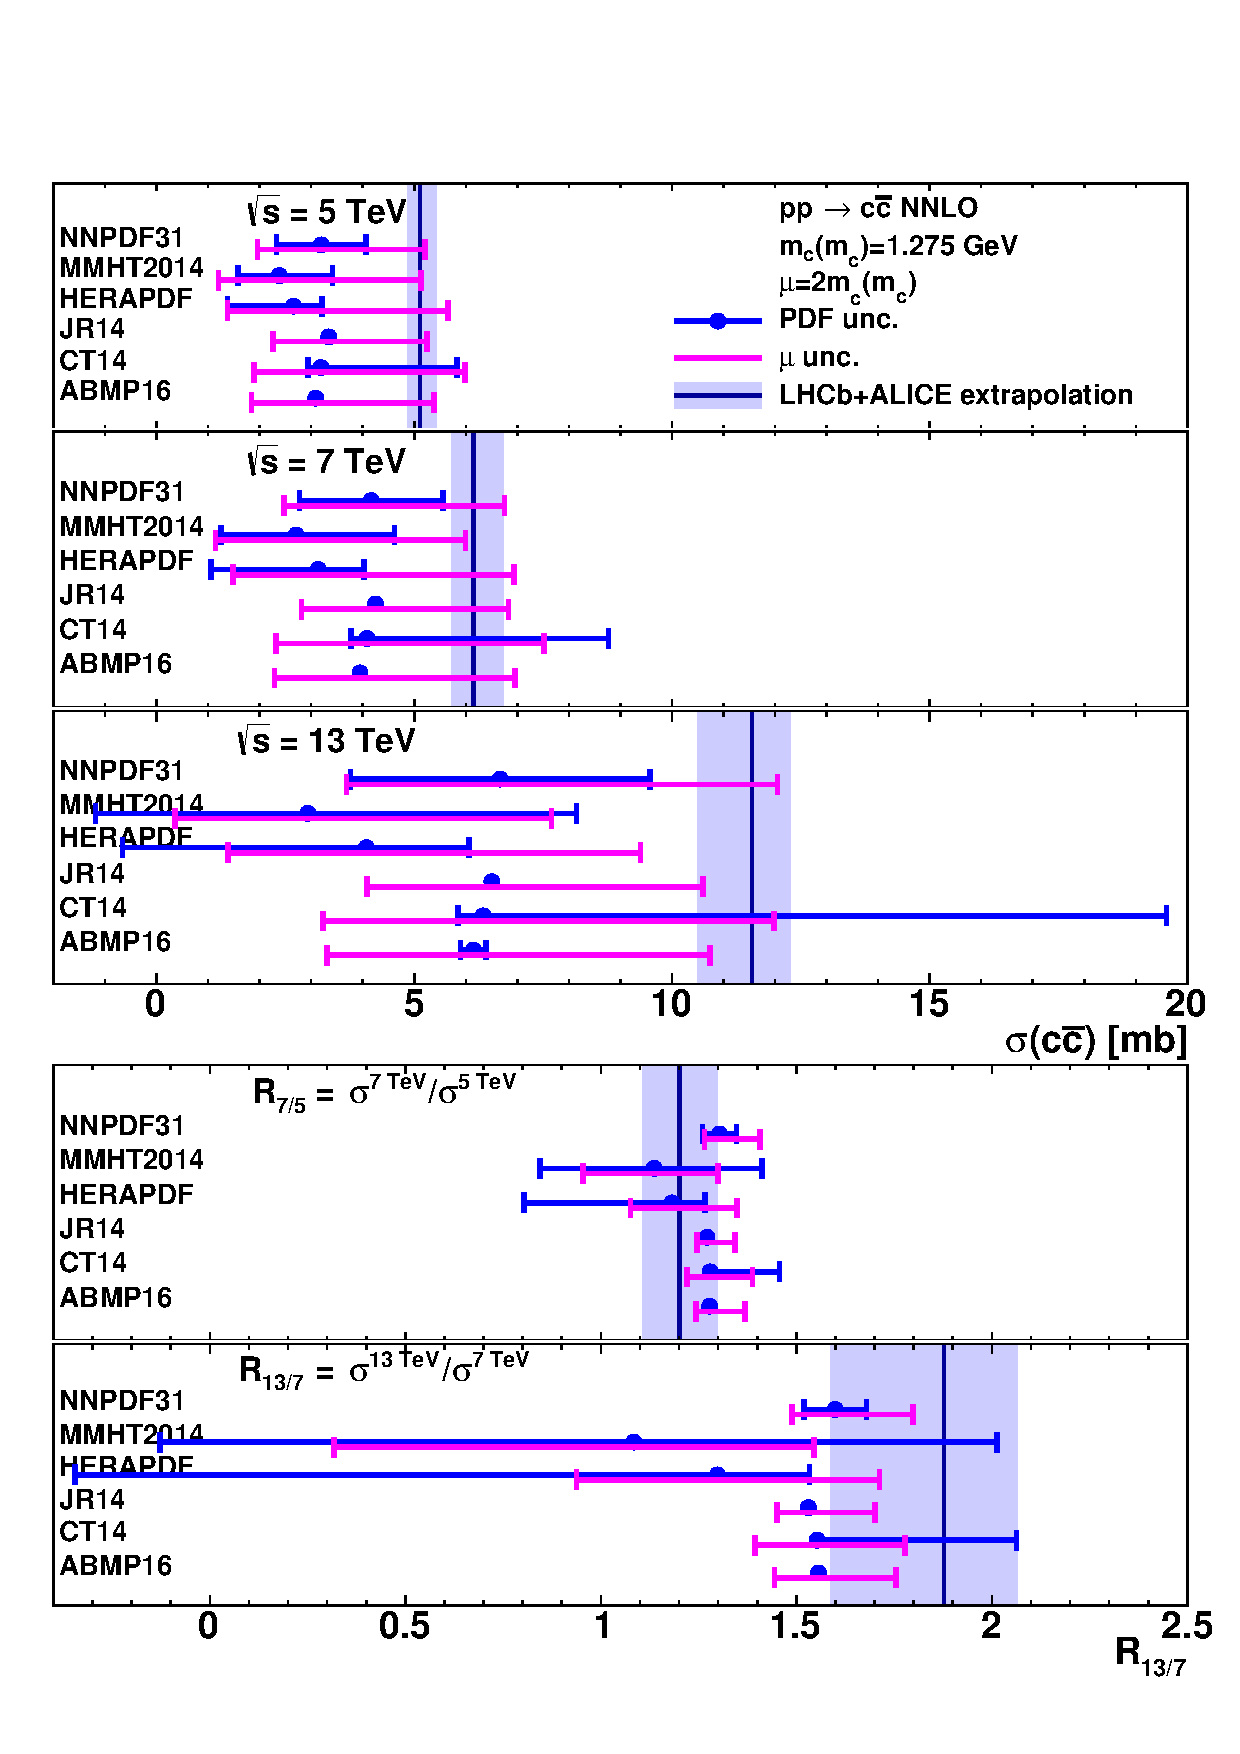
\includegraphics[width=1.0\textwidth]{figs/plot5.pdf}
    \caption{Comparison of the extrapolated total charm production cross sections and their ratios with the NNLO theoretical predictions using different PDF sets.}
    \label{fig:extrap}
\end{figure}

To demonstrate the feasibility of the provided observables to constrain the PDFs, we employ a profiling technique~\cite{Paukkunen:2014zia} based on minimizing $\chi^2$ function between data and theoretical predictions taking into account both data and theoretical uncertainties arising from PDF variations. The analysis is performed using the xFitter program~\cite{Alekhin:2014irh}. We consider the MMHT2014 PDF set and the ratios $R_{7/5}$ and $R_{13/7}$ which exhibit least scale uncertainties. The correlation of $R_{7/5}$ and $R_{13/7}$ because of the common input 7 TeV data sets is taken into account. The PDF uncertainties are included in $\chi^2$ through nuisance parameters, and the values of these nuisance parameters at the minimum are interpreted as optimised (or profiled) PDFs, while their uncertainties determined using the tolerance criterion of $\Delta\chi^2 = 1$ correspond to the new PDF uncertainties. The original and profiled MMHT2014 gluon PDF is shown in Fig.~\ref{fig:extrap-profile} at the scale $Q^2 = 10$ and $100$~GeV$^2$. The profiled distribution exhibits greatly reduced uncertainties at low $x$, and in this region the distribution is shifted towards larger values of the gluon density.

\begin{figure}
    \centering
    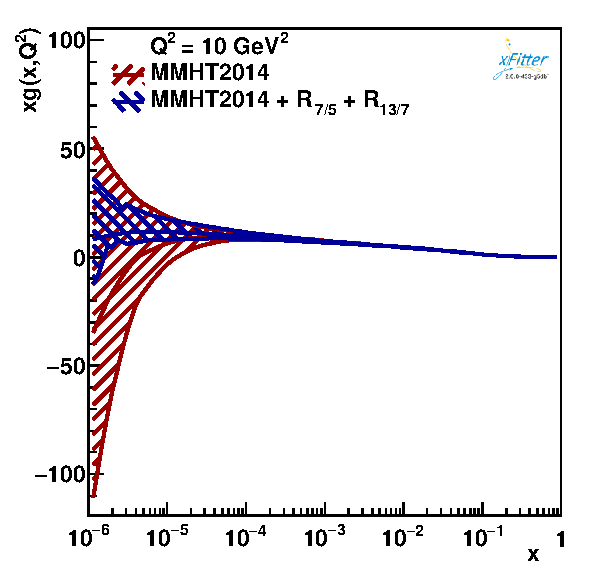
\includegraphics[width=0.49\textwidth]{figs/q2_10_pdf_g.pdf}
    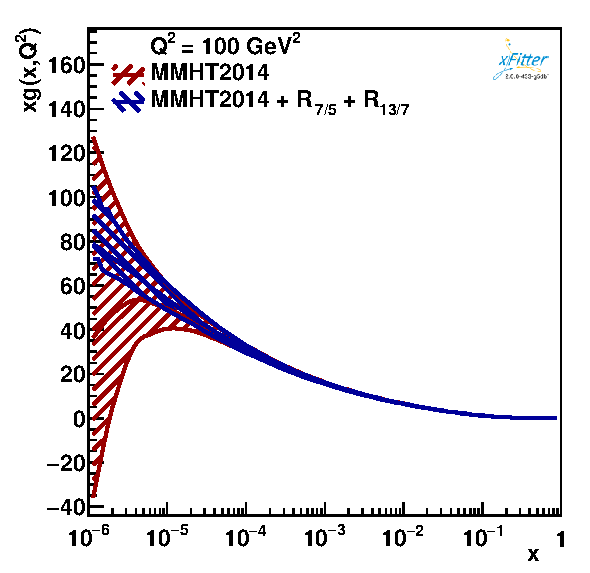
\includegraphics[width=0.49\textwidth]{figs/q2_100_pdf_g.pdf}
    \caption{The gluon distribution of the original and profiled MMHT2014 set at $Q^2 = 10$~GeV$^2$ (left) and $Q^2 = 100$~GeV$^2$ (right).}
    \label{fig:extrap-profile}
\end{figure}

\subsection{Prompt neutrino fluxes}

....Discussion at qualitative level about reduction of uncertainties.
\\
\\

\section{Conclusions}
\label{conclu}


\subsection*{Acknowledgments}
We thank John Campbell for help in porting the routines we developed for
the computation of charm hadroproduction using $\overline{\rm MS}$ mass 
(processes $pp$ $\rightarrow$ $c\bar{c}$ and $pp$ $\rightarrow$ $b\bar{b}$) 
to the last public version of MCFM. 
This work is partially supported by grants.....

\section*{Appendix: description of the routines added to MCFM}
...name of routines, what they do, how to compile.... 

\cleardoublepage
\newpage

\bibliographystyle{JHEP} 
\bibliography{papercharmrun}

\end{document}

